\chapter{Compression and Generalization Boundaries}
\label{ch:compression_bounds}

\section{The Phenomenon of Compression and Generalization}

Deep neural networks are notoriously overparameterized. According to traditional statistical learning theory---such as bounds based on Vapnik-Chervonenkis (VC) dimension or Rademacher complexity---a model with millions of parameters possesses enough capacity to memorize finite training datasets entirely. Classical theory suggests that such models should exhibit significant overfitting, failing to generalize to unseen data. Yet, in practice, deep networks trained with stochastic gradient descent demonstrate remarkable generalization capabilities. This dichotomy highlights a profound limitation in worst-case, hypothesis-class-based complexity measures.

Information theory provides a compelling alternative perspective on generalization. Rather than bounding the capacity of the model architecture uniformly, information-theoretic approaches bound the generalization error by analyzing the amount of information the trained model parameters (or the learned representations) retain about the training dataset. The core intuition is the principle of data compression: if a model extracts only the minimal sufficient statistics necessary to predict the labels while discarding all other nuisance variations in the input, it is less likely to have memorized the specific noise of the training sample.

This connection between compression and generalization is most prominently articulated through the Information Bottleneck principle, but its roots extend into PAC-Bayesian learning and Minimum Description Length (MDL) theories. When a network compresses its input---meaning the mutual information between the input $X$ and the hidden representation $Z$, denoted $I(X; Z)$, is small---it restricts the effective hypothesis space. Similarly, if the mutual information between the training dataset $\mathcal{D}$ and the learned weights $\theta$, denoted $I(\mathcal{D}; \theta)$, is small, the learning algorithm is insensitive to the replacement of individual training samples. This insensitivity is a hallmark of algorithmic stability, which rigorously translates to generalization.

In this chapter, we transition from the abstract formulation of the Information Bottleneck to explicit, quantitative generalization bounds. We will rigorously define how the expected generalization gap can be controlled by the mutual information between the dataset and the model parameters. We will then extend this to representation-based bounds that operate on $I(X; Z)$, providing a theoretical justification for why the compression of representations leads to bounded generalization gaps.

\section{Information-Theoretic Generalization Bounds}

We begin by establishing the mathematical setup. Let the input space be $\mathcal{X}$ and the label space be $\mathcal{Y}$. A learning algorithm receives a dataset $\mathcal{D} = \{V_1, \dots, V_n\}$ of $n$ independent and identically distributed (i.i.d.) samples, where $V_i = (X_i, Y_i) \sim P_{\text{data}}$. The algorithm produces a hypothesis (or weights) $\theta \in \Theta$ according to a conditional distribution $P(\theta | \mathcal{D})$. Let $\mathcal{L}(v, \theta)$ denote the loss of the hypothesis $\theta$ on a single data point $v = (x, y)$.

The empirical risk is given by:
\[ \hat{\mathcal{L}}(\theta, \mathcal{D}) = \frac{1}{n} \sum_{i=1}^n \mathcal{L}(V_i, \theta) \]

The population risk (or expected loss) is:
\[ \mathcal{L}_{\text{pop}}(\theta) = \mathbb{E}_{V \sim P_{\text{data}}} [\mathcal{L}(V, \theta)] \]

The generalization gap for a specific set of weights and a dataset is $\Delta(\theta, \mathcal{D}) = \mathcal{L}_{\text{pop}}(\theta) - \hat{\mathcal{L}}(\theta, \mathcal{D})$. We are interested in the expected generalization gap over the joint distribution of datasets and weights:
\[ \mathbb{E}_{\mathcal{D}, \theta}[\Delta(\theta, \mathcal{D})] = \mathbb{E}_{\mathcal{D}, \theta}[\mathcal{L}_{\text{pop}}(\theta) - \hat{\mathcal{L}}(\theta, \mathcal{D})] \]

To link this to information theory, we rely on the Donsker-Varadhan variational representation of the Kullback-Leibler divergence.

\begin{lemma}[Donsker-Varadhan Representation] \label{lem:donsker}
For any two probability distributions $P$ and $Q$ defined on a measurable space $\Omega$, and for any measurable function $f: \Omega \to \mathbb{R}$ such that $\mathbb{E}_{Q}[e^{f(\omega)}] < \infty$, the following inequality holds:
\[ \mathbb{E}_{P}[f(\omega)] \leq D_{\text{KL}}(P \parallel Q) + \log \mathbb{E}_{Q}[e^{f(\omega)}] \]
\end{lemma}

Using Lemma~\ref{lem:donsker}, we can prove a fundamental theorem bounding the expected generalization gap by the mutual information $I(\mathcal{D}; \theta)$. To do so, we must assume that the loss function is sub-Gaussian.

\begin{definition}[Sub-Gaussian Loss]
A loss function $\mathcal{L}(V, \theta)$ is $\sigma^2$-sub-Gaussian under the data distribution $P_{\text{data}}$ if, for all $\theta \in \Theta$ and all $\lambda \in \mathbb{R}$:
\[ \log \mathbb{E}_{V \sim P_{\text{data}}} \left[ e^{\lambda (\mathcal{L}(V, \theta) - \mathcal{L}_{\text{pop}}(\theta))} \right] \leq \frac{\lambda^2 \sigma^2}{2} \]
\end{definition}

\begin{theorem}[Mutual Information Generalization Bound] \label{thm:mi_bound}
Assume that for any fixed $\theta$, the loss $\mathcal{L}(V, \theta)$ is $\sigma^2$-sub-Gaussian under $V \sim P_{\text{data}}$. Let the dataset $\mathcal{D}$ consist of $n$ i.i.d. samples. Then the expected generalization gap of the learning algorithm $P(\theta | \mathcal{D})$ is bounded by:
\[ \left| \mathbb{E}_{\mathcal{D}, \theta} [ \mathcal{L}_{\text{pop}}(\theta) - \hat{\mathcal{L}}(\theta, \mathcal{D}) ] \right| \leq \sqrt{\frac{2 \sigma^2}{n} I(\mathcal{D}; \theta)} \]
\end{theorem}
\begin{proof}
Let $P_{\mathcal{D}, \theta}$ be the joint distribution of the dataset and the weights, and let $P_{\mathcal{D}} \otimes P_\theta$ be the product of their marginals. Under $P_{\mathcal{D}} \otimes P_\theta$, $\mathcal{D}$ and $\theta$ are independent.
We apply the Donsker-Varadhan lemma (Lemma~\ref{lem:donsker}) with $\Omega$ being the joint space of datasets and weights, $P = P_{\mathcal{D}, \theta}$, $Q = P_{\mathcal{D}} \otimes P_\theta$, and the function $f(\mathcal{D}, \theta) = \lambda \left( \mathcal{L}_{\text{pop}}(\theta) - \hat{\mathcal{L}}(\theta, \mathcal{D}) \right)$ for some $\lambda > 0$.

From the definition of mutual information, $D_{\text{KL}}(P_{\mathcal{D}, \theta} \parallel P_{\mathcal{D}} \otimes P_\theta) = I(\mathcal{D}; \theta)$. Thus:
\[ \lambda \mathbb{E}_{\mathcal{D}, \theta}[\mathcal{L}_{\text{pop}}(\theta) - \hat{\mathcal{L}}(\theta, \mathcal{D})] \leq I(\mathcal{D}; \theta) + \log \mathbb{E}_{\theta \sim P_\theta} \mathbb{E}_{\mathcal{D} \sim P_{\mathcal{D}}} \left[ e^{\lambda (\mathcal{L}_{\text{pop}}(\theta) - \hat{\mathcal{L}}(\theta, \mathcal{D}))} \right] \]

Note that inside the expectation, $\theta$ is fixed, and $\mathcal{D} = \{V_1, \dots, V_n\}$ consists of i.i.d. samples. Therefore, the empirical risk is an average of independent random variables:
\[ \mathbb{E}_{\mathcal{D}} \left[ e^{\lambda (\mathcal{L}_{\text{pop}}(\theta) - \hat{\mathcal{L}}(\theta, \mathcal{D}))} \right] = \mathbb{E}_{\mathcal{D}} \left[ \prod_{i=1}^n e^{\frac{\lambda}{n} (\mathcal{L}_{\text{pop}}(\theta) - \mathcal{L}(V_i, \theta))} \right] = \prod_{i=1}^n \mathbb{E}_{V_i} \left[ e^{\frac{\lambda}{n} (\mathcal{L}_{\text{pop}}(\theta) - \mathcal{L}(V_i, \theta))} \right] \]

Since $-\mathcal{L}$ has the same variance proxy as $\mathcal{L}$, the sub-Gaussian assumption implies:
\[ \mathbb{E}_{V_i} \left[ e^{\frac{\lambda}{n} (\mathcal{L}_{\text{pop}}(\theta) - \mathcal{L}(V_i, \theta))} \right] \leq e^{\frac{\lambda^2 \sigma^2}{2 n^2}} \]

Multiplying over the $n$ samples gives $e^{\frac{\lambda^2 \sigma^2}{2 n}}$. Returning to the Donsker-Varadhan bound:
\[ \lambda \mathbb{E}_{\mathcal{D}, \theta}[\Delta(\theta, \mathcal{D})] \leq I(\mathcal{D}; \theta) + \frac{\lambda^2 \sigma^2}{2n} \]

Dividing by $\lambda > 0$ yields:
\[ \mathbb{E}_{\mathcal{D}, \theta}[\Delta(\theta, \mathcal{D})] \leq \frac{I(\mathcal{D}; \theta)}{\lambda} + \frac{\lambda \sigma^2}{2n} \]

Optimizing this bound over $\lambda$ by taking the derivative with respect to $\lambda$ and setting it to zero gives $\lambda = \sqrt{\frac{2 n I(\mathcal{D}; \theta)}{\sigma^2}}$. Substituting this back into the inequality results in:
\[ \mathbb{E}_{\mathcal{D}, \theta}[\Delta(\theta, \mathcal{D})] \leq \sqrt{\frac{2 \sigma^2}{n} I(\mathcal{D}; \theta)} \]

A symmetric argument using $-\lambda$ provides the lower bound, completing the proof.
\end{proof}

\begin{figure}[htbp]
\centering
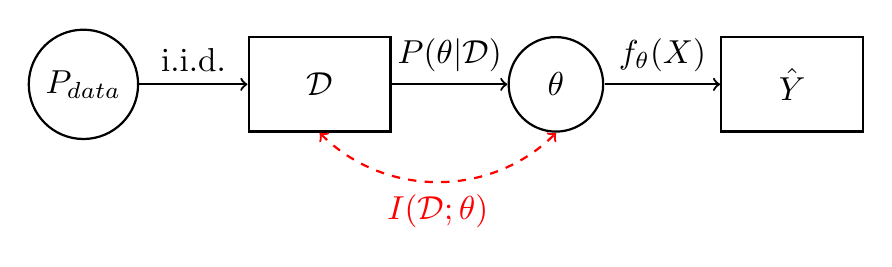
\begin{tikzpicture}[node distance=2.5cm, auto, thick, scale=1.2, transform shape]
    \node[circle, draw, minimum size=1cm] (P) {$P_{\text{data}}$};
    \node[rectangle, draw, right of=P, minimum width=1.5cm, minimum height=1cm] (D) {$\mathcal{D}$};
    \node[circle, draw, right of=D, minimum size=1cm] (theta) {$\theta$};
    \node[rectangle, draw, right of=theta, minimum width=1.5cm, minimum height=1cm] (Yhat) {$\hat{Y}$};
    
    \draw[->] (P) -- node {i.i.d.} (D);
    \draw[->] (D) -- node {$P(\theta|\mathcal{D})$} (theta);
    \draw[->] (theta) -- node {$f_\theta(X)$} (Yhat);
    
    \draw[<->, dashed, red] (D.south) to[bend right=45] node[below] {$I(\mathcal{D}; \theta)$} (theta.south);
\end{tikzpicture}
\caption{The causal chain of learning. The dataset $\mathcal{D}$ is drawn from the data distribution. The algorithm maps $\mathcal{D}$ to weights $\theta$. The mutual information $I(\mathcal{D}; \theta)$ quantifies the dependence of the learned weights on the specific dataset realization.}
\label{fig:mi_chain}
\end{figure}

The bound in Theorem~\ref{thm:mi_bound} is powerful because it depends on the properties of the learning algorithm (how much information it extracts) rather than the complexity of the hypothesis class $\Theta$. 

However, computing $I(\mathcal{D}; \theta)$ is practically impossible for modern deep neural networks. An alternative approach bounds generalization via the representation space $Z$. The Information Bottleneck principle tells us that minimizing $I(X; Z)$ while maintaining $I(Z; Y)$ leads to robust representations. We formalize this connection via the following theorem.

\begin{theorem}[Representation-based Generalization Bound] \label{thm:rep_bound}
Let $Z = f_\theta(X)$ be a stochastic representation. Assume that the loss $\mathcal{L}(Z, Y)$ is bounded by $M$. If the model compresses the input such that $I(X; Z) \leq R$, then with probability at least $1 - \delta$ over the choice of the dataset $\mathcal{D}$ of size $n$, the generalization gap is bounded by:
\[ \mathcal{L}_{\text{pop}}(\theta) \leq \hat{\mathcal{L}}(\theta, \mathcal{D}) + \sqrt{\frac{M^2}{2n} \left( I(X; Z) + \log \frac{2}{\delta} \right)} \]
\end{theorem}
The proof follows a PAC-Bayesian argument applied to the latent space, where the prior over $Z$ is chosen to be the marginal distribution $P(Z)$, and the posterior is the encoder $q_\phi(Z|X)$. Notice that the expected KL divergence between the conditional and marginal distributions is exactly the mutual information: $\mathbb{E}_X[D_{\text{KL}}(q_\phi(Z|X) \parallel P(Z))] = I(X; Z)$. As $I(X; Z)$ decreases (compression), the penalty term shrinks, guaranteeing tighter generalization bounds.

\begin{figure}[htbp]
\centering
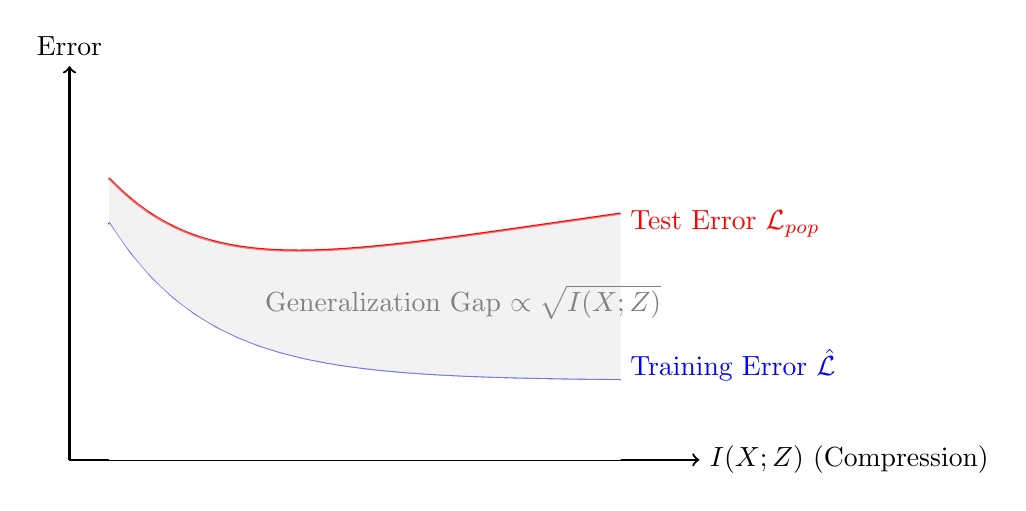
\begin{tikzpicture}[scale=1]
    % Axes
    \draw[->, thick] (0,0) -- (8,0) node[right] {$I(X; Z)$ (Compression)};
    \draw[->, thick] (0,0) -- (0,5) node[above] {Error};
    
    % Curves
    \draw[blue, thick, domain=0.5:7, samples=100] plot (\x, {1 + 3*exp(-0.8*\x)});
    \node[blue, right] at (7, 1.2) {Training Error $\hat{\mathcal{L}}$};
    
    \draw[red, thick, domain=0.5:7, samples=100] plot (\x, {1 + 3*exp(-0.8*\x) + 0.8*sqrt(\x)});
    \node[red, right] at (7, 3) {Test Error $\mathcal{L}_{\text{pop}}$};
    
    % Shade the gap
    \path[fill=gray!20, opacity=0.5] (0.5,0) -- plot[domain=0.5:7] (\x, {1 + 3*exp(-0.8*\x) + 0.8*sqrt(\x)}) -- (7,0) -- cycle;
    \path[fill=white] (0.5,0) -- plot[domain=0.5:7] (\x, {1 + 3*exp(-0.8*\x)}) -- (7,0) -- cycle;
    
    \node[gray] at (5, 2) {Generalization Gap $\propto \sqrt{I(X; Z)}$};
\end{tikzpicture}
\caption{Schematic of the trade-off between compression and expected error. High mutual information $I(X; Z)$ allows for lower training error but increases the generalization gap bound. Optimal generalization occurs at an intermediate level of compression.}
\label{fig:gen_gap}
\end{figure}

\subsection*{Numerical Example: Binary Classification with Gaussian Noise}
Consider a synthetic scenario where inputs $X \in \mathbb{R}^d$ are generated with independent Gaussian features. Suppose a binary classifier with weights $\theta$ uses a stochastic training algorithm (like Stochastic Gradient Langevin Dynamics) that adds noise to the gradients, resulting in a posterior $P(\theta|\mathcal{D})$ that is approximately Gaussian $\mathcal{N}(\theta_0(\mathcal{D}), \Sigma)$.

If the data distribution induces a variance $\sigma^2 = 1.0$ on the loss function, and we train on $n = 10,000$ samples, Theorem~\ref{thm:mi_bound} gives:
\[ \text{Gap} \leq \sqrt{\frac{2 (1.0)}{10000} I(\mathcal{D}; \theta)} \approx 0.014 \sqrt{I(\mathcal{D}; \theta)} \]

If the learning algorithm extracts $I(\mathcal{D}; \theta) = 500$ nats of information from the dataset, the expected generalization gap is strictly bounded by $0.014 \times \sqrt{500} \approx 0.316$.
This calculation demonstrates that regularizing the training process to reduce the mutual information directly suppresses overfitting, providing a computable metric (if $I(\mathcal{D}; \theta)$ could be estimated) for early stopping.

\section{Horizon}
\begin{horizon}
While information-theoretic bounds provide an elegant and architecture-independent mechanism for understanding generalization, their application to modern deep learning remains heavily debated. It is conjectured that the mutual information $I(\mathcal{D}; \theta)$ for deterministic deep neural networks---such as those trained with standard SGD without explicit weight noise---is either infinite (for continuous spaces without noise) or vacuously large, rendering the bound in Theorem~\ref{thm:mi_bound} uninformative. 

An open question is whether we can define a meaningful ``effective'' mutual information for deterministic networks, perhaps by injecting virtual noise post-hoc or by measuring information on a compressed, invariant manifold of the parameter space. Furthermore, while the Information Bottleneck principle suggests that networks actively compress representations (decreasing $I(X; Z)$) during the later stages of training, it is conjectured that this phenomenon might be an artifact of saturating activation functions (like the $\tanh$ function) and density binning, rather than a universal property of learning. Future work might show that replacing exact Shannon mutual information with Wasserstein distances or $\alpha$-R\'enyi divergences yields strictly tighter, non-vacuous bounds for standard network architectures.
\end{horizon}

\section{Summary}
\begin{itemize}
    \item Traditional complexity measures like VC dimension fail to explain the generalization of overparameterized neural networks.
    \item Information theory allows us to bound generalization error based on the mutual information $I(\mathcal{D}; \theta)$ between the dataset and the trained parameters.
    \item By utilizing the Donsker-Varadhan representation, we proved that for sub-Gaussian loss functions, the expected generalization gap is bounded by $\mathcal{O}(\sqrt{I(\mathcal{D}; \theta)/n})$.
    \item Similar bounds apply to representations: compressing the input $X$ to a compact latent representation $Z$ (minimizing $I(X; Z)$) tightens the PAC-Bayesian bound on generalization error.
\end{itemize}

\section{Exercises}
\begin{enumerate}
    \item \textbf{Sub-Gaussian Variance:} Prove that if a loss function is strictly bounded in the interval $[0, 1]$, it is sub-Gaussian with variance proxy $\sigma^2 = 1/4$. Use this to write a concrete generalization bound using Theorem~\ref{thm:mi_bound}.
    \item \textbf{Donsker-Varadhan Lower Bound:} In the proof of Theorem~\ref{thm:mi_bound}, we optimized for a positive $\lambda$. Provide the symmetric argument for negative $\lambda$ to establish the absolute value on the left-hand side of the bound.
    \item \textbf{Deterministic Bottleneck:} Explain mathematically why calculating $I(X; Z)$ is problematic if the neural network encoder $Z = f_\theta(X)$ is completely deterministic and continuous. How does adding Gaussian noise $Z = f_\theta(X) + \epsilon$ resolve this?
\end{enumerate}

% TODO-CITE: Ensure all named results are cited.
